% Basic setup. Most papers should leave these options alone.
\documentclass[fleqn,usenatbib]{mnras}

% MNRAS is set in Times font. If you don't have this installed (most LaTeX
% installations will be fine) or prefer the old Computer Modern fonts, comment
% out the following line
%\usepackage{newtxtext,newtxmath}
% Depending on your LaTeX fonts installation, you might get better results with one of these:
\usepackage{mathptmx}
%\usepackage{txfonts}

% Use vector fonts, so it zooms properly in on-screen viewing software
% Don't change these lines unless you know what you are doing
\usepackage[T1]{fontenc}
\usepackage{ae,aecompl}


%%%%% AUTHORS - PLACE YOUR OWN PACKAGES HERE %%%%%

% Only include extra packages if you really need them. Common packages are:
\usepackage{savesym}
\usepackage{amsmath}
\savesymbol{iint}
\usepackage{txfonts}
\restoresymbol{TXF}{iint}

\usepackage{graphicx}	% Including figure files
%\usepackage{amsmath}	% Advanced maths commands
\usepackage{amssymb}	% Extra maths symbols
\usepackage[ansinew]{inputenc}
\usepackage{amsfonts}
\usepackage{graphicx}
\usepackage{epsfig}
\usepackage{color}
\usepackage[normalem]{ulem}
\usepackage{natbib}
%\usepackage{url}
\usepackage{hyperref}
\usepackage{placeins}
\usepackage{caption}
\usepackage{subcaption}
\captionsetup{compatibility=false}

% By default the URLs are put in typewriter type in the body and the
% bibliography of the document when using the \url command.  If you are
% using many long URLs you may want to uncommennt the next line so they
% are typeset a little smaller.
%\renewcommand{\UrlFont}{\small\tt}

\def\aap{{A\&A}}
\def\AaA{{A\&A}}
\def\AJ{{AJ}}
\def\aj{{AJ}}
\def\ApJ{{ApJ}}
\def\apj{{ApJ}}
\def\apjl{{ApJL}}
\def\ApJL{{ApJL}}
\def\ApJSupp{{ApJS}}
\def\MN{{MNRAS}}
\def\mnras{{MNRAS}}
\def\pasp{{PASP}}
\def\jcap{JCAP}
\def\pasj{{PASJ}}
\def\nat{Nature}
\def\ARAA{{ARA\&A}}
\def\apjs{{ApJS}}
\def\araa{{ARA\&A}}
\def\apss{{Ap\&SS}}
\def\cjaa{{ChJAA}}
\def\aaps{{A\&AS}}

\newcommand{\eg}{{e.g., }}
\newcommand{\ie}{{i.e., }}

\pdfminorversion=5

\title[Dreaming of Photo-z's]{Applying Deep Learning to the Image Photo-z Problem}

\author[S. E. Thrush and R. J. Brunner]{
  Samantha E. Thrush$^1$\thanks{thrush2@illinois.edu} and Robert J.~Brunner$^{1,2,3,4}$ \\
$^1$Department of Astronomy, University of Illinois, Urbana, IL 61801 USA\\
$^2$Department of Physics, University of Illinois, Urbana, IL 61801 USA\\
$^3$Department of Statistics, University of Illinois, Champaign, IL 61820 USA\\
$^4$National Center for Supercomputing Applications, Urbana, IL 61801 USA
}

% These dates will be filled out by the publisher
\date{Accepted XXX. Received YYY; in original form ZZZ}

% Enter the current year, for the copyright statements etc.
\pubyear{2015}

% Don't change these lines
\begin{document}
\label{firstpage}
\pagerange{\pageref{firstpage}--\pageref{lastpage}}
\maketitle

\begin{abstract}
When large data sets of galaxies are collected, their associated redshifts are usually collected by finding their photometric redshifts, which takes additional time for a survery to complete.  However, if deep learning via deep convolutional neural networks (ConvNets) are utilized, photometric redshifts of galaxies can be predicted without the need for photometry to be completed by the associated survey. In this paper, we present an application of ConvNets on reduced and pixelated galaxy images and redshift data from the Sloan Digital Sky Survey (SDSS).  We will show that ConvNets are able to accurately predict the redshift of a sample galaxy image in a way that is competitive with previous works on this subject.
\end{abstract}

\begin{keywords}
methods: data analysis -- techniques: image processing -- methods: statistical
-- surveys -- galaxies:statistics.
\end{keywords}

\section{Introduction}
  \label{sec:introduction}

HERE IS AN EXAMPLE OF NORMAL TEXT. HERE IS AN EXAMPLE OF A CITED PIECE OF TEXT~\citep{ross2011ameliorating,seo2012acoustic}.

IN ORDER TO START A NEW PARAGRAPH, THERE MUST BE A BLANK LINE IN BETWEEN TWO PARAGRAPHS.

HERE I REFER TO A SECTION BY NAME IN LATEX, AKA SECTION~\ref{sec:data}.

\section{Data}
  \label{sec:data}

\subsection{Sloan Digital Sky Survey}
  \label{sec:sdss}

\begin{figure}
  \centering
  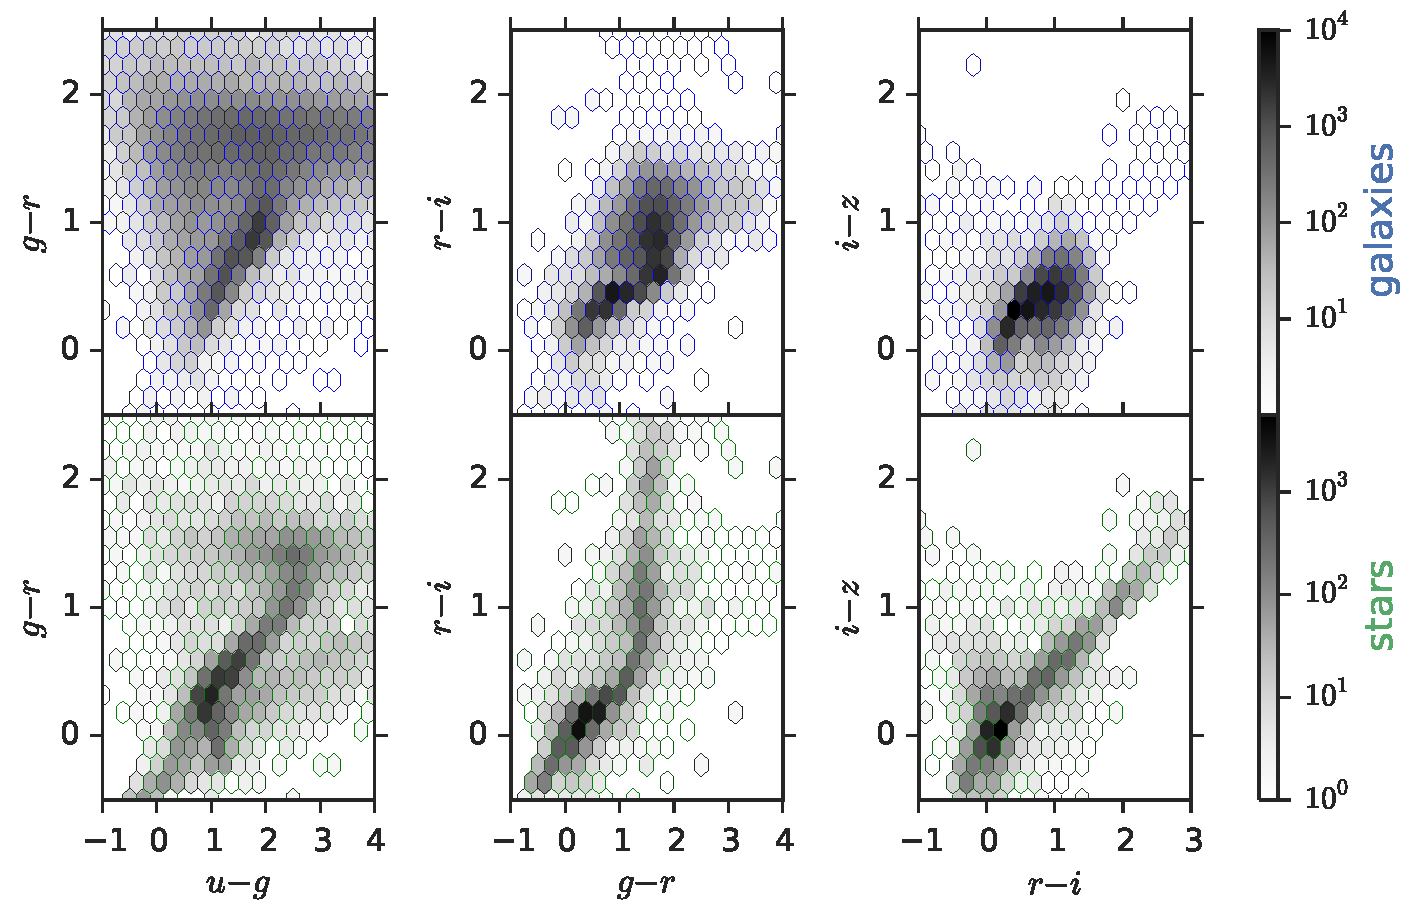
\includegraphics[width=\columnwidth]{figures/sdss_color_color.pdf}
  \caption{
    Hexbin plots showing the color-color space distribution of galaxies (blue, top row) and stars (green, bottom row)
    in the SDSS data set used in this analysis.
    It is easy to see that there is significant overlap between stars
    and galaxies in these color-color spaces. 
  }
  \label{fig:sdss_color_color}
\end{figure}

TEXT AFTER A FIGURE. HERE IS AN EXAMPLE OF A FOOT NOTE\footnote{http://skyserver.sdss.org/casjobs/}.

AN EXAMPLE OF "COMPUTER-LOOKING" TEXT: (\texttt{zWarning = 0})

AN EXAMPLE OF ITALICIZED TEXT: $r$ 

AN EXAMPLE OF THE "TIMES" OPERATOR BETWEEN TWO NUMBERS: $48\times48$ pixels
with luptitude values in each pixel.

AN EQUATION PRESENTED INLINE WITH THE TEXT: $10.7 < r < 23.1$,
and the galaxies in this sample have a mean redshift of $z \sim 0.36$.
The $ugriz$ color-color space of the sample is plotted in
Figure~\ref{fig:sdss_color_color}.

The first two panels of Figure~\ref{fig:sdss_mag} show the number of objects
and the fraction of stars in the test set as functions of $r$-band magnitude.
Similarly, Figure~\ref{fig:sdss_g_r} shows the number of objects and the
fraction of stars in the test set as functions of $g-r$ color.

We do not show the distributions for the training and validation sets in
Figures~\ref{fig:sdss_mag} and \ref{fig:sdss_g_r} to avoid cluttering the
plots.


\subsection{Canada-France-Hawaii Telescope Lensing Survey}

\begin{figure}
  \centering
  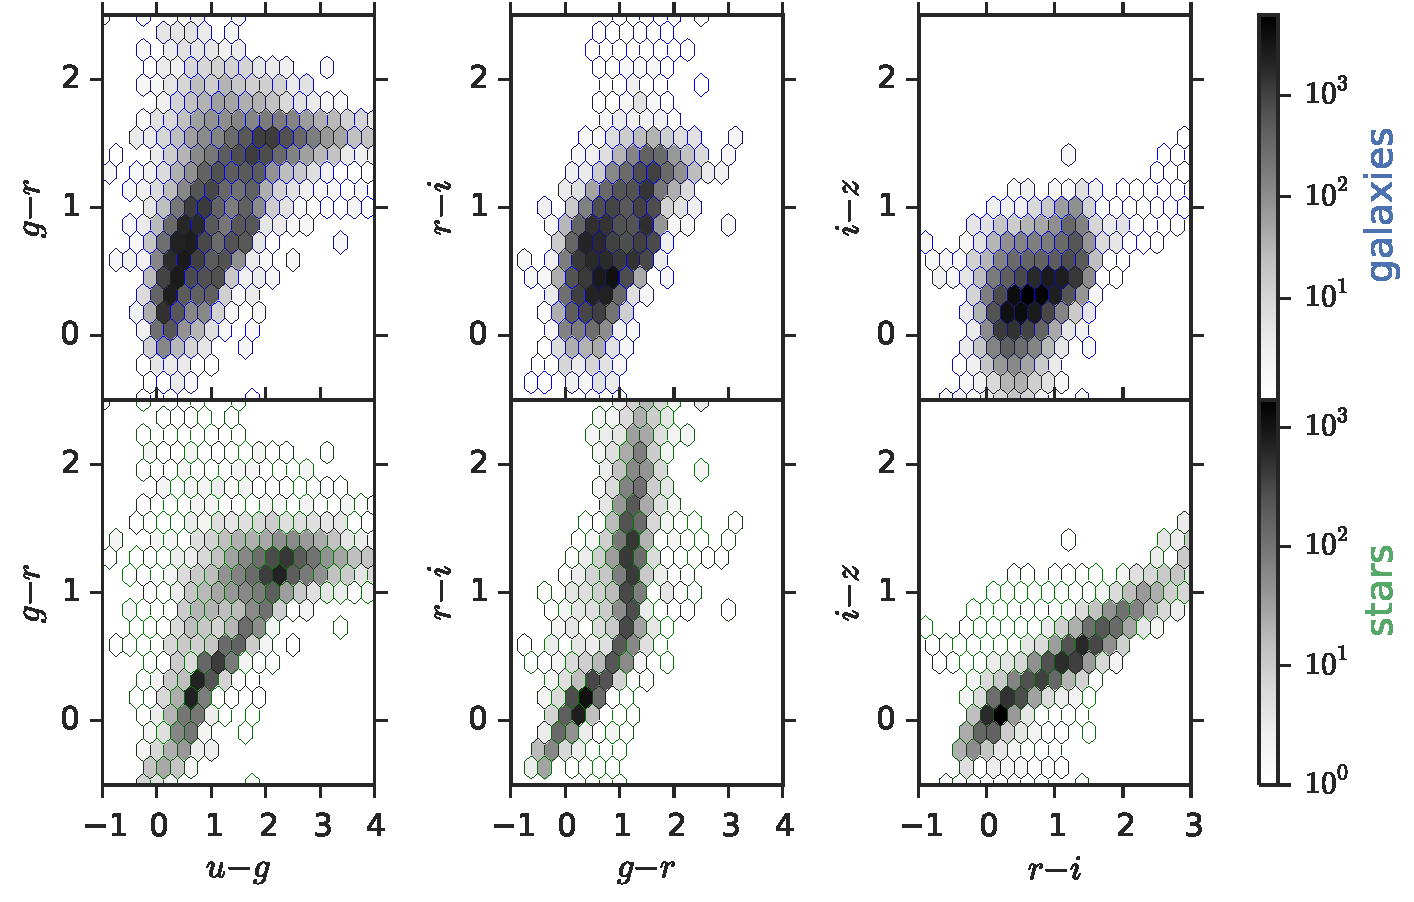
\includegraphics[width=\columnwidth]{figures/clens_color_color.pdf}
  \caption{
    Hexbin plots showing the color-color space distribution of
    galaxies (blue, top row) and stars (green, bottom row)
    in the CFHTLenS data set used in this analysis.
  }
  \label{fig:clens_color_color}
\end{figure}

We also use photometric data from
the Canada-France-Hawaii Telescope Lensing Survey
\cite[CFHTLenS\footnote{http://www.cfhtlens.org/};][]
{heymans2012cfhtlens,erben2013cfhtlens,hildebrandt2012cfhtlens}.

\section{Deep Learning}
  \label{sec:deep_learning}

\subsection{Neural Networks}

\begin{figure*}
  \centering
  \begin{subfigure}[]{0.49\linewidth}
    \centering
    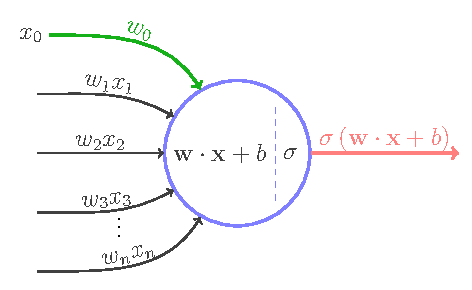
\includegraphics[width=0.6\textwidth]{figures/neuron.pdf}
    \caption{}
    \label{fig:neuron_a}
  \end{subfigure}
  \begin{subfigure}[]{0.49\linewidth}
    \centering
    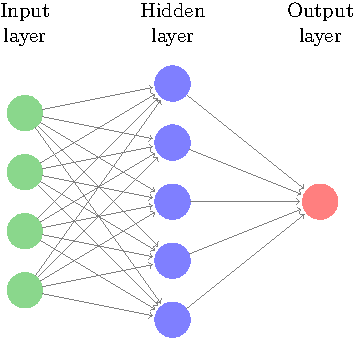
\includegraphics[width=0.6\textwidth]{figures/network.pdf}
    \caption{}
    \label{fig:neuron_b}
  \end{subfigure}
  \caption{
    (a) A mathematical model of a biological neuron.
    (b) A schematic diagram of a neural network with one hidden layer.
    }
\end{figure*}

An artificial neuron in most artificial neural networks is represented
as a mathematical function that models a biological neural structure
(Figure~\ref{fig:neuron_a}).
Let $\bmath{x}=\left(x_1,x_2,\dots,x_n\right)$ be a vector of inputs to a given neuron,
$\bmath{w}=\left(w_1,w_2,\dots,w_n\right)$ be a vector of weights, and
$b$ be the bias.
Then, the output of the neuron is
\begin{equation}
  y = \sigma \left( \bmath{w} \cdot \bmath{x} + b \right),
  \label{eq:neuron_output}
\end{equation}
where $\sigma$ is the activation function (or \textit{non-linearity}).

A schematic representation is shown in Figure~\ref{fig:neuron_b}.

The gradients in \ref{eq:neuron_output} can be computed using the
\textit{backpropagation} procedure~\citep{rumelhart1988learning},

\begin{align}
  \frac{ \partial L }{ \partial y_i } &= y_i - \hat{y}_i \\
  \frac{ \partial L }{ \partial x_i } &=
    \frac{ \partial L }{ \partial y_i }
    \frac{ \partial y_i }{ \partial x_i }.
\end{align}
At each hidden layer, the derivative of the loss function with respect to the
output of each unit is a weighted sum of the derivatives with respect to the
inputs of the subsequent layer,
\begin{align}
  \frac{ \partial L }{ \partial y_j } &=
    \sum_{i} w_{ji} \frac{ \partial L }{ \partial x_i}   \\
  \frac{ \partial L }{ \partial x_j } &=
    \frac{ \partial L }{ \partial y_j }
    \frac{ \partial y_j }{ \partial x_j }.
\end{align}
Finally, once the gradients $\partial L / \partial x_j$ have been
computed, it is straightforward to compute the gradients for the weight,
\begin{equation}
\frac{\partial L}{\partial w_{jk}} = y_k \frac{\partial L}{\partial x_j}.
\end{equation}

\subsection{Convolutional Neural Networks}
  \label{sec:convnet}

Mathematically, we replace the dot product in Equation~\ref{eq:neuron_output}
with a sum of convolutions. Thus, the $k$-th feature map is given by
\begin{equation}
  y^k = \sigma \left( \sum_{m} \bmath{w}_m^k \ast \bmath{x}_m + b^k \right),
\end{equation}
where we sum over the set of input feature maps,
$\ast$ is the convolution operator, and $\bmath{w}_m^k$ represent the filters.


\subsection{Neural Network Architecture}

\begin{table*}
  \centering
  \caption{Summary of ConvNet architecture and hyperparameters. Note that pooling layers have no learnable parameters.}
  \label{table:hyperparamters}
  \begin{tabular}{ccccccc}
    \hline
    type            & filters & filter size & padding & non-linearity & initial weights & initial biases \\
    \hline
    convolutional   & 32          & $5\times5$  & -       & leaky ReLU    & orthogonal      & 0.1            \\
    convolutional   & 32          & $3\times3$  & 1       & leaky ReLU    & orthogonal      & 0.1            \\
    pooling         & -           & $2\times2$  & -       & -             & -               & -              \\
    convolutional   & 64          & $3\times3$  & 1       & leaky ReLU    & orthogonal      & 0.1            \\
    convolutional   & 64          & $3\times3$  & 1       & leaky ReLU    & orthogonal      & 0.1            \\
    convolutional   & 64          & $3\times3$  & 1       & leaky ReLU    & orthogonal      & 0.1            \\
    pooling         & -           & $2\times2$  & -       & -             & -               & -              \\
    convolutional   & 128         & $3\times3$  & 1       & leaky ReLU    & orthogonal      & 0.1            \\
    convolutional   & 128         & $3\times3$  & 1       & leaky ReLU    & orthogonal      & 0.1            \\
    convolutional   & 128         & $3\times3$  & 1       & leaky ReLU    & orthogonal      & 0.1            \\
    pooling         & -           & $2\times2$  & -       & -             & -               & -              \\
    fully-connected & 2048        & -           & -       & leaky ReLU    & orthogonal      & 0.01            \\
    fully-connected & 2048        & -           & -       & leaky ReLU    & orthogonal      & 0.01            \\
    fully-connected & 2           & -           & -       & softmax       & orthogonal      & 0.01            \\
    \hline
  \end{tabular}
\end{table*}

We present the overall architecture of our ConvNet model in Table~\ref{table:hyperparamters}.

The architecture of \cite{krizhevsky2012imagenet}
uses relatively large receptive fields ($11\times11$) in the first convolutional layers.
\citet{zeiler2014visualizing} and \cite{dieleman2015rotation}
also use large receptive fields of $7\times7$ and $6\times6$
in the first convolution layer, respectively.

In the interest of scientific reproducibility, we make all our code available
at \href{https://github.com/EdwardJKim/dl4astro}{https://github.com/EdwardJKim/dl4astro}.


\section{Reducing Overfitting}
  \label{sec:overfitting}
  
Our convolution neural network has $11\times10^6$ learnable parameters,
while there are only $4\times10^4$ images in the training set.

\subsection{Data Augmentation}
  \label{sec:data_augmentation}
  
One common method to combat overfitting is to artificially increase
the number of training data by using label-preserving
transformations~\citep{krizhevsky2012imagenet,dieleman2015rotation,dieleman2016exploiting}.
Each image is transformed as follows:
\begin{itemize}
\item{Rotation: 
Rotating an image does not change whether the object is a star or a galaxy.
We exploit this rotational symmetry and randomly rotate each image by a multiple of
$90^{\circ}$. }

\item{Reflection:
We flip each image horizontally with a probability of 0.5 to exploit mirror symmetry. }
\item{Translation:
We also have translational symmetry in the images.
Given an image of size $48\times48$ pixels, we extract a random contiguous crop
of size $44\times44$.
Each cropping is equivalent to randomly shifting a $44\times44$ image by up to 4 pixels
vertically and/or horizontally. }
\item{Gaussian noise:
We introduce random Gaussian noise to each pixel values
by using a similar method to \cite{krizhevsky2012imagenet}. }
\end{itemize}
These data augmentation schemes add almost no computational cost,
as they are performed on the CPU while the GPU is training the ConvNets on images.

\subsection{Dropout}

We use a regularization technique called dropout~\citep{hinton2012improving}
in the fully-connected layers.

\subsection{Model Combination}
  \label{sec:bmc}

The posterior probability that a source is a galaxy is given by
\begin{equation} \label{eq:posterior_bmc}
  P \left(G | \bmath{x}, \bmath{D}, \bmath{M}, \bmath{E} \right)
  = \sum_{e \in \bmath{E}} P \left(G | \bmath{x}, \bmath{M}, e \right)
  P \left(e | \bmath{D} \right),
\end{equation}
where $\bmath{x}$ is the input, $\bmath{D}$ is the data set,
$\bmath{M}$ is the set of models (\ie different transformations of input images),
and $e$ is an element in the ensemble space $\bmath{E}$ of possible model combinations.
By Bayes' Theorem, the posterior probability of $e$ given $\bmath{D}$ is given by
\begin{equation} \label{eq:p_ensemble}
  P \left(e | \bmath{D} \right)
  = \frac{P \left(e \right)}{P \left(\bmath{D} \right)}
  \prod_{d \in \bmath{D}} P \left( d | e \right)
  \propto P \left(e\right) \prod_{d \in \bmath{D}} P \left(d | e \right).
\end{equation}

For probabilistic classifiers,
we can directly use the probabilistic predictions
and write Equation~\ref{eq:p_ensemble} as
\begin{equation} \label{eq:p_ensemble_prob}
  P \left( e | \bmath{D} \right) \propto 
  P \left( e \right) \prod_{i=1}^{N}
  \hat{y}_i y_i + 
  \left(1 - \hat{y}_i\right) \left(1 - y_i\right).
\end{equation}


\section{Trees for Probabilistic Classifications}
  \label{sec:tpc}
  
TPC is a part of a publicly available software package called
\textsc{MLZ}\footnote{http://pythonhosted.org/MLZ/}
(Machine Learning for Photo-$z$).

\begin{equation} \label{eq:information_gain}
  I_G \left(D_{\rmn{node}}, X\right)
  = I_d \left( D_{\rmn{node}} \right)
  - \sum_{x \in \rmn{values}(X)}
  \frac{|D_{\rmn{node}, x}|}{|D_{\rmn{node}}|}
  I_d \left( D_{\rmn{node}, x} \right),
\end{equation}

\noindent
where $D_{\rmn{node}}$ is the training data in a given node,
$X$ is one of the possible dimensions (\eg magnitudes or colors)



\section{Results and Discussion}
  \label{sec:results_and_discussion}

In this section, we first describe the performance metrics that were used for
evaluating the models.

\subsection{Classification Metrics}

\begin{table}
  \caption{The definition of the classification performance metrics.}
  \centering
  \begin{tabular}{c l}
  \hline
  Metric & Meaning \\
  \hline
  AUC & Area under the Receiver Operating Curve \\
  MSE & Mean squared error \\
  $c_g$ & Galaxy completeness \\
  $p_g$ & Galaxy purity \\
  $c_s$ & Star completeness \\
  $p_s$ & Star purity \\
  $p_g(c_g=x)$ & Galaxy purity at $x$ galaxy completeness \\
  $c_s(p_s=x)$ & Star completeness at $x$ star purity \\
  $CAL$ & Calibration error with overlapping binning \\
  $\mid\Delta N_g\mid / N_g$ & Absolute error in number of galaxies\\
  \hline
  \end{tabular}
  \label{table:metrics}
\end{table}

Probabilistic classification models can be considered as
functions that output a probability estimate of each source
to be in one of the classes (\eg a star or a galaxy).

\subsubsection{Receiver Operating Characteristic Curve}

When we have no information about the operating condition
when evaluating the performance of classifiers,
there are effective tools such as
the Receiver Operating Characteristic (ROC) curve
\citep*{swets2000better}.

\subsubsection{Completeness and Purity}

We define the galaxy \textit{completeness}
$c_g$ (also known as recall or sensitivity) as
the fraction of the number of true galaxies classified as galaxies
out of the total number of true galaxies,

\subsubsection{Mean Squared Error}

We also use the mean squared error
(MSE; also known as the Brier score~\citep{brier1950verification})
as a performance metric. We define MSE as
\begin{equation} \label{eq:mse}
  \rmn{MSE} = \frac{1}{N} \sum^{N}_{j=1}
  \left( y_j - \hat{y}_j \right)^2,
\end{equation}
The MSE can be considered as both a score function that quantifies
how well a set of probabilistic predictions is calibrated,
or a loss function.

\subsubsection{Calibration Error}

A fully probabilistic classifier predicts not only the class label,
but also its confidence level on the prediction.

\subsubsection{Number of galaxies}

Ideally, the probabilistic output of a classifier would be used in subsequent
scientific analyses.

\subsection{CFHTLenS}
  \label{sec:results_cfht}

\begin{table*}
  \caption{
    A summary of the classification performance metrics
    as applied to the CFHTLenS data.
    The definition of the metrics is summarized in Table~\ref{table:metrics}.
    The bold entries highlight the best performance values within each column.
  }
  \centering
  \begin{tabular}{l c c c c c c}
    \hline
    classifier & AUC & MSE & $p_{g}(c_g=0.96)$ & $c_{s}(p_s=0.97)$ & CAL & $ |\Delta N_g|/N_g$ \\
    \hline
    ConvNet                       & \textbf{0.9948} & 0.0112          & \textbf{0.9972} & 0.8971          & \textbf{0.0197}  & \textbf{0.0029} \\
    TPC${}_{\rmn{morph}}$         & 0.9924          & \textbf{0.0109} & 0.9963          & \textbf{0.9268} & 0.0245           & 0.0056 \\
    TPC${}_{\rmn{phot}}$          & 0.9876          & 0.0189          & 0.9927          & 0.8044          & 0.0266           & 0.0101 \\
    \hline
  \end{tabular}
  \label{table:clens_metrics}
\end{table*}

\begin{figure}
  \centering
  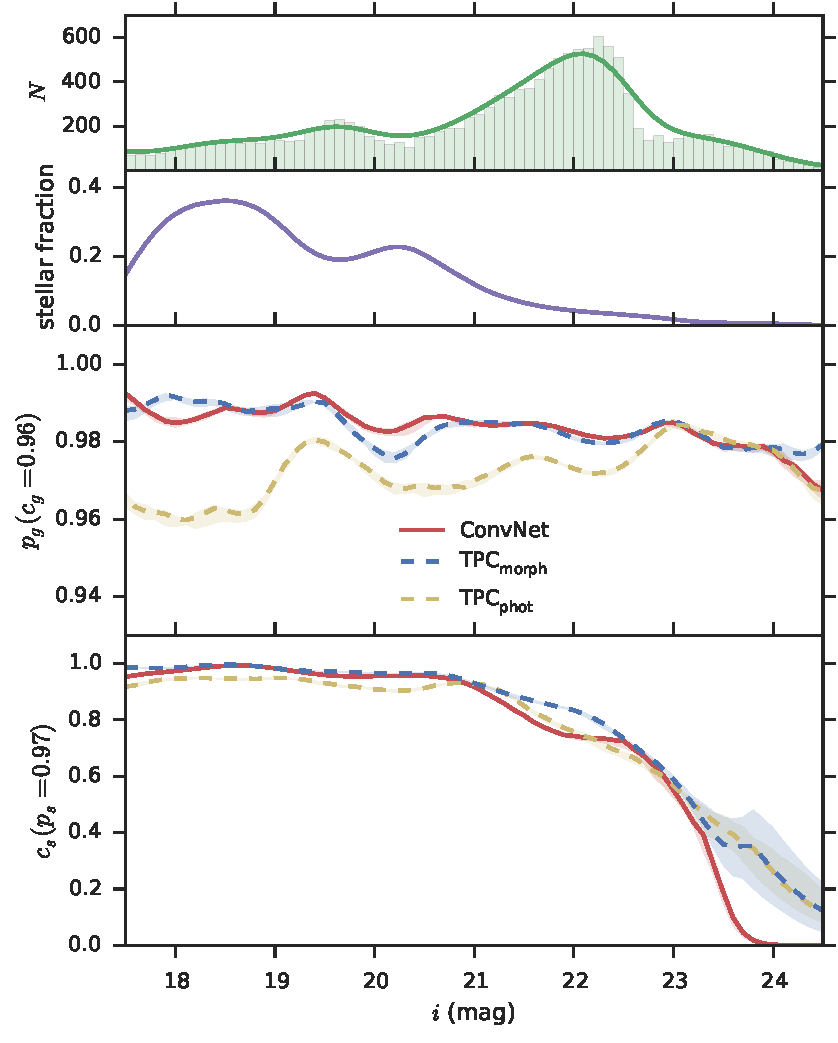
\includegraphics[width=\columnwidth]{figures/clens_mag.pdf}
  \caption{Galaxy purity and star completeness values as functions
           of the $i$-band magnitude (differential counts)
           as estimated by kernel density estimation (KDE)
           in the CFHTLenS data set.
           The top panel shows the histogram with a bin size of 0.1 mag
           and the KDE for objects in the test set.
           The second panel shows the fraction of stars estimated by KDE
           as a function of magnitude.
           The bottom two panels compare the galaxy purity and star completeness
           values for ConvNet (red solid line),
           $\rmn{TPC}_{\rmn{morph}}$ (blue dashed line),
           and $\rmn{TPC}_{\rmn{phot}}$ (yellow dashed line)
           as functions of magnitude.
           The $1 \sigma$ confidence bands are estimated by
           bootstrap sampling.}
  \label{fig:clens_mag}
\end{figure}

\begin{figure}
  \centering
  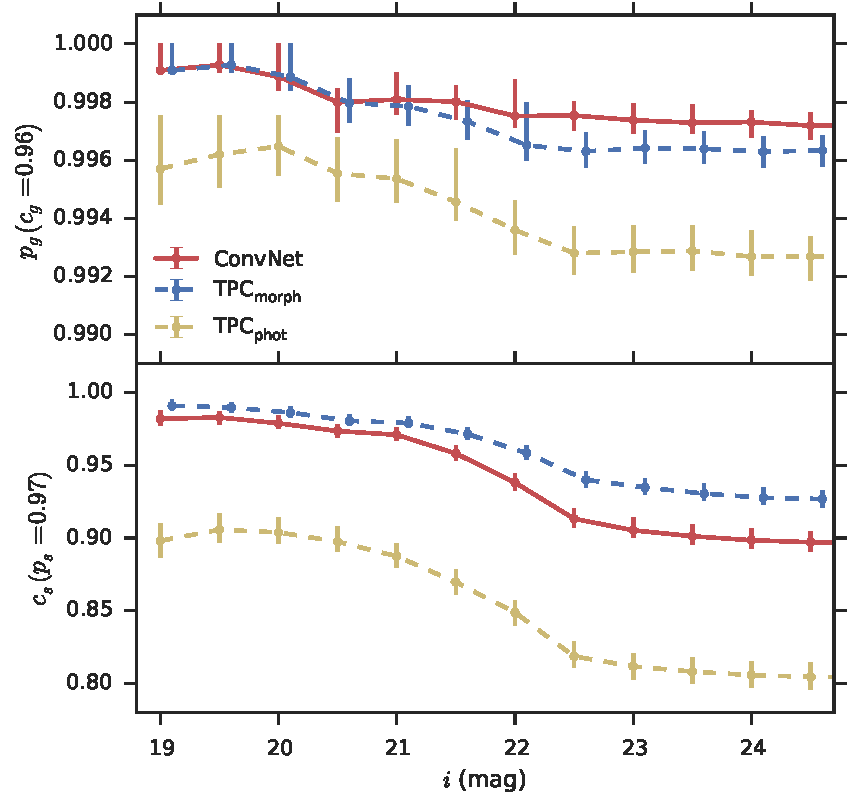
\includegraphics[width=\columnwidth]{figures/clens_integrated.pdf}
  \caption{
    Galaxy purity and star completeness as functions of the $i$-band
    magnitude (integrated counts) in the CFHTLenS data set.
    The upper panel compares the galaxy
    purity values for ConvNet (red solid line), $\rmn{TPC}_{\rmn{morph}}$
    (blue dashed line), and $\rmn{TPC}_{\rmn{phot}}$ (yellow dashed line).
    The lower panel compares the star completeness values.
    The $1 \sigma$ error bars are computed following the method
    of \citet{paterno2004calculating} to avoid the unphysical
    errors of binomial or Poisson statistics.
    }
  \label{fig:clens_integrated}
\end{figure}

\begin{figure}
  \centering
  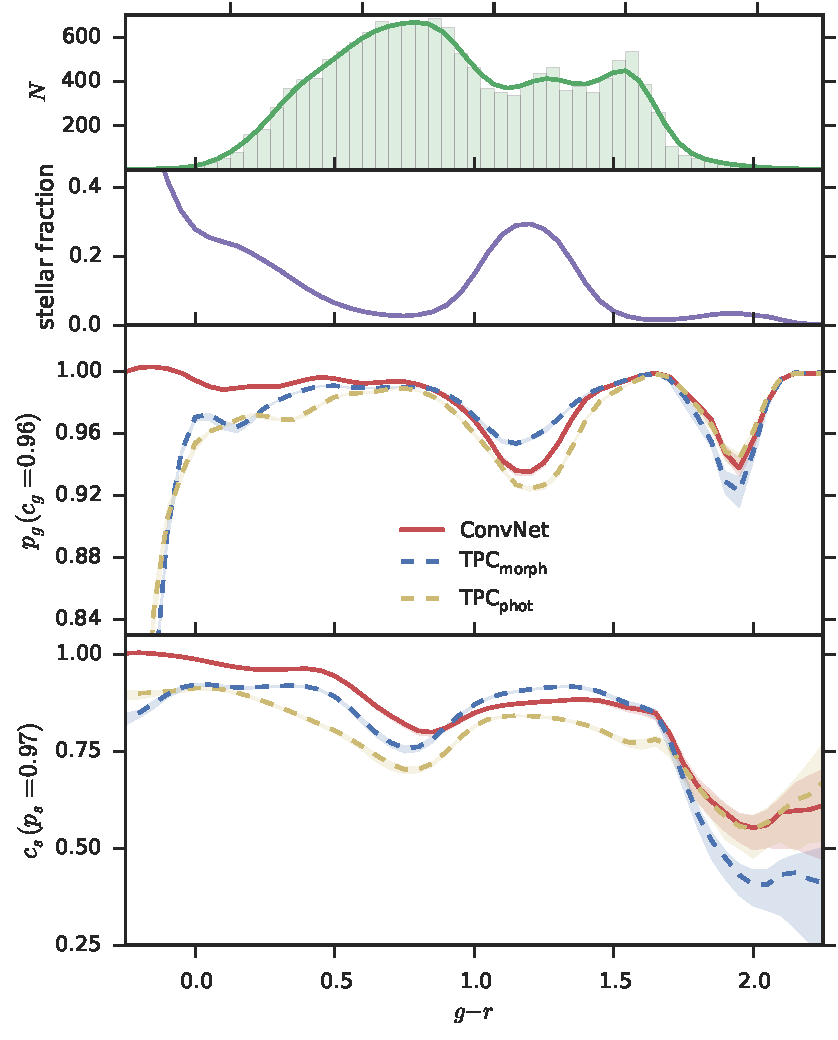
\includegraphics[width=\columnwidth]{figures/clens_g_r.pdf}
  \caption{Similar to Figure~\ref{fig:clens_mag}
           but as a function of $g-r$ color.
           The bin size of histogram in the top panel is 0.05.}
  \label{fig:clens_g_r}
\end{figure}

\begin{figure*}
  \centering
  \begin{minipage}[c]{0.49\textwidth}
    \centering
    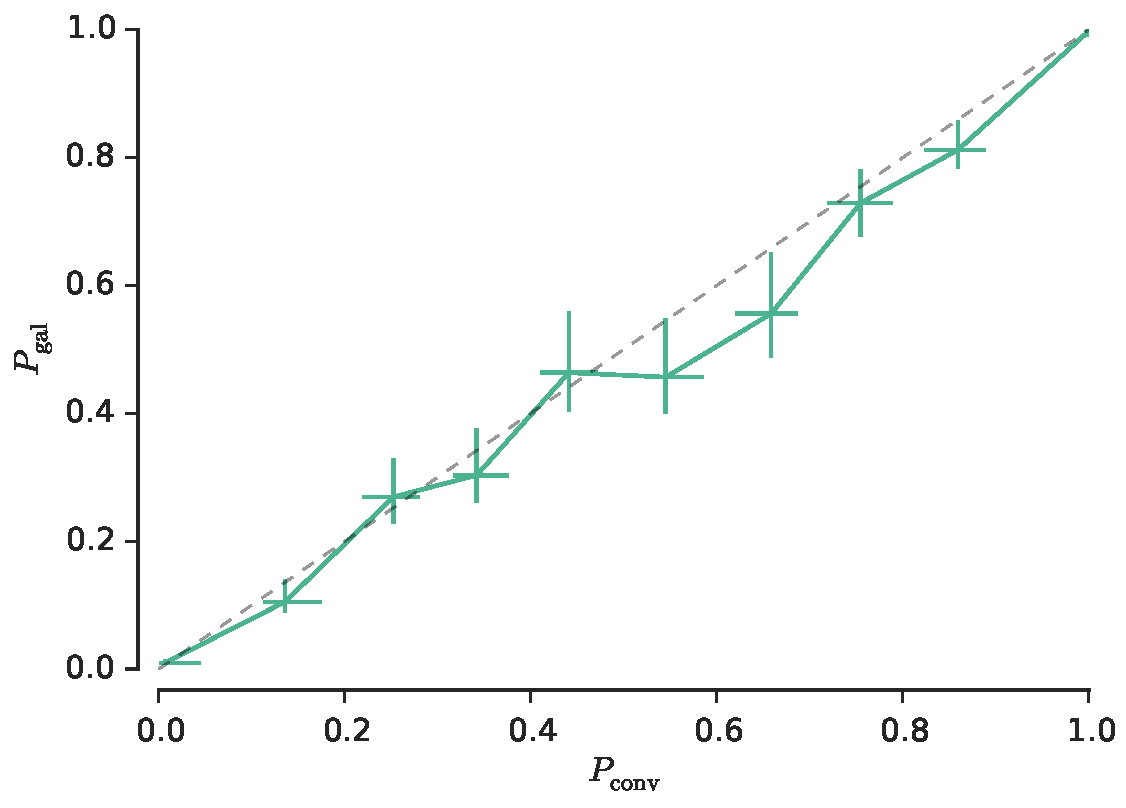
\includegraphics[width=\textwidth]{figures/clens_calibration_conv.pdf}
    \caption{
      The calibration curve for ConvNet as applied to the CFHTLenS data set.
      $P_{\rmn{gal}}$ is the fraction of objects that are galaxies, and
      $P_{\rmn{conv}}$ is the probabilistic output generated by ConvNet.
      The dashed line displays the relationship
      $P_{\rmn{gal}} = P_{\rmn{conv}}$.
      The $1 \sigma$ error bars are computed following the method
      of \citet{paterno2004calculating}.
      }
    \label{fig:clens_calibration_conv}
  \end{minipage}
  \hfill
  \begin{minipage}[c]{0.49\textwidth}
    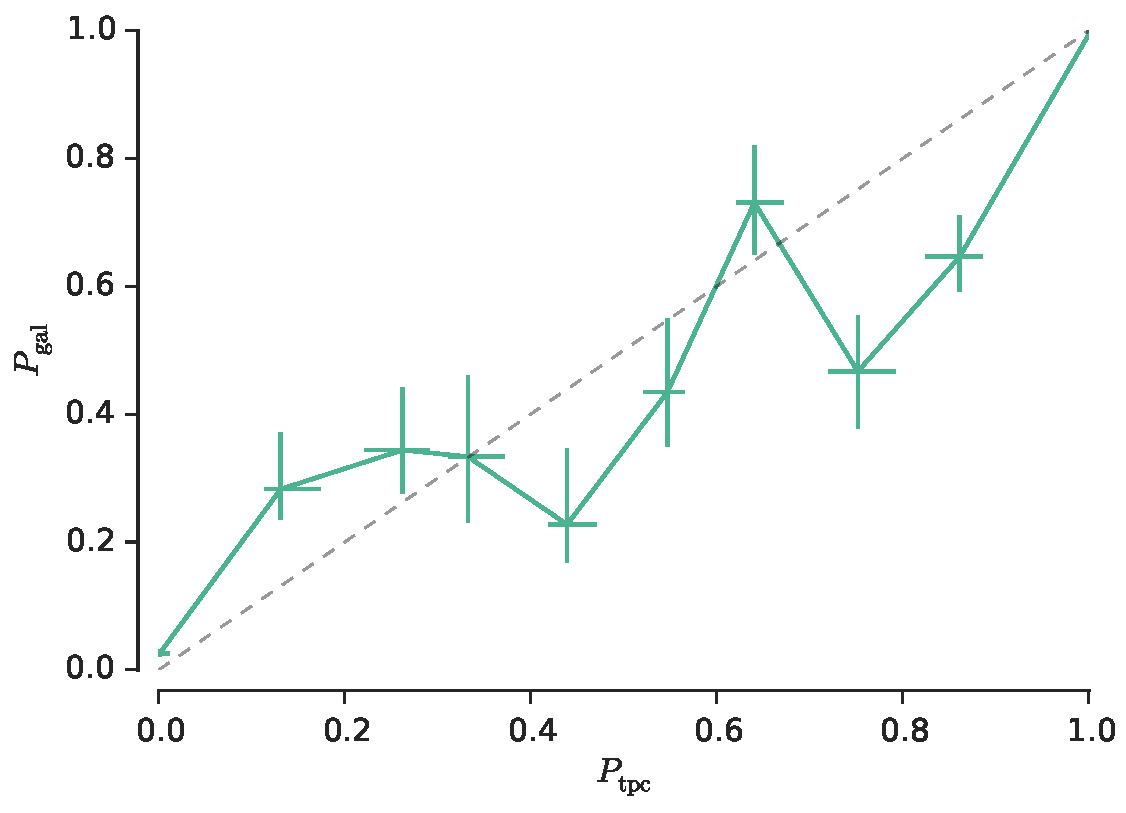
\includegraphics[width=\textwidth]{figures/clens_calibration_tpc.pdf}
    \caption{Similar to Figure~\ref{fig:clens_calibration_conv} but for
      $\rmn{TPC}_{\rmn{morph}}$.
      $P_{\rmn{tpc}}$ is the probabilistic output generated by $\rmn{TPC}_{\rmn{morph}}$.}
    \label{fig:clens_calibration_tpc}
  \end{minipage}
\end{figure*}

\begin{figure*}
  \centering
  \begin{subfigure}[c]{0.24\linewidth}
  \centering
    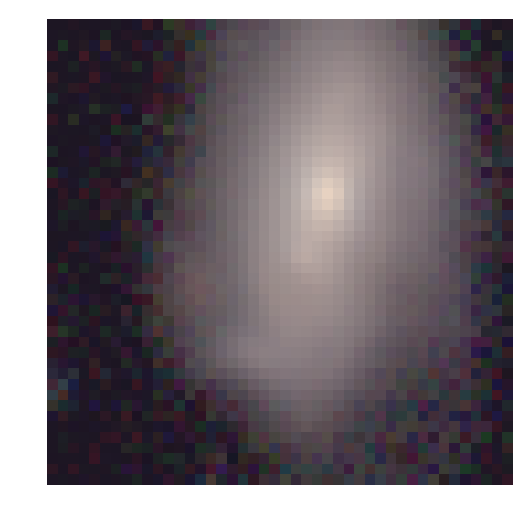
\includegraphics[width=\textwidth]{figures/galaxy_original.pdf}
    \caption{Input (5 bands$\times44\times44$)}
  \end{subfigure}
  \hfill
  \begin{subfigure}[c]{0.24\linewidth}
  \centering
    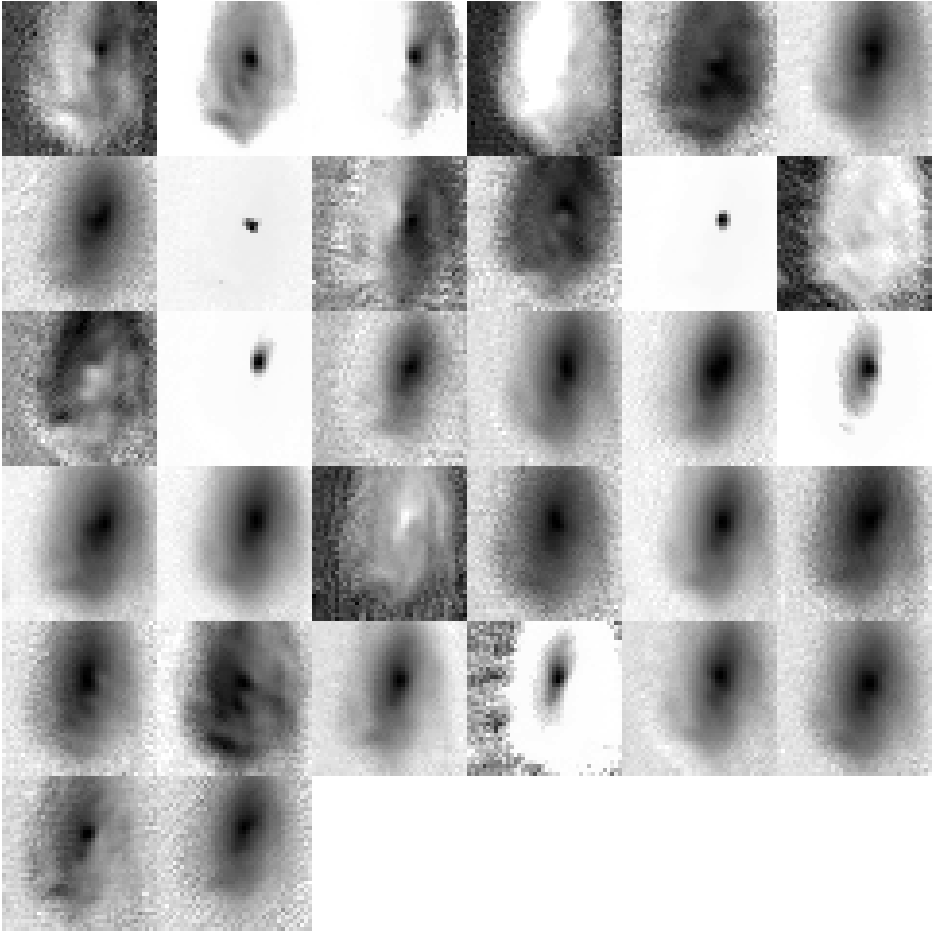
\includegraphics[width=\textwidth]{figures/galaxy_conv11.pdf}
    \caption{Layer 1 (32 maps$\times40\times40$)}
  \end{subfigure}
  \hfill
  \begin{subfigure}[c]{0.24\linewidth}
  \centering
    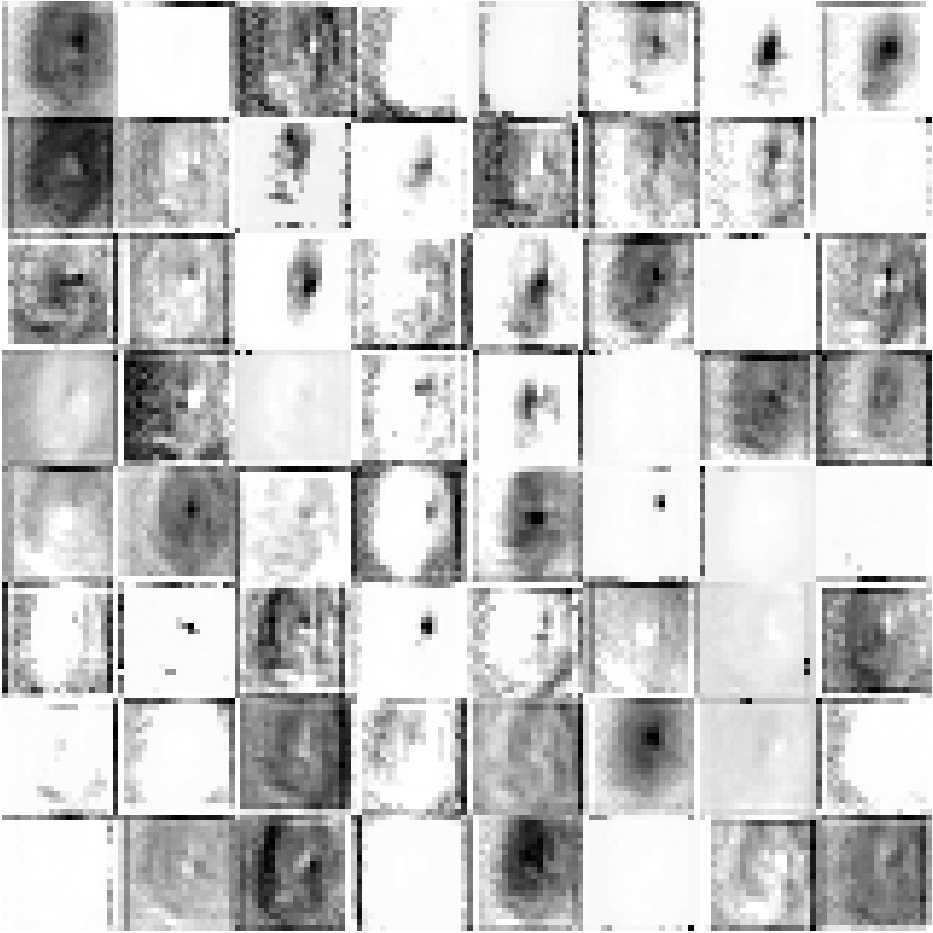
\includegraphics[width=\textwidth]{figures/galaxy_conv21.pdf}
    \caption{Layer 3 (64 maps$\times20\times20$)}
  \end{subfigure}
  \hfill
  \begin{subfigure}[c]{0.24\linewidth}
  \centering
    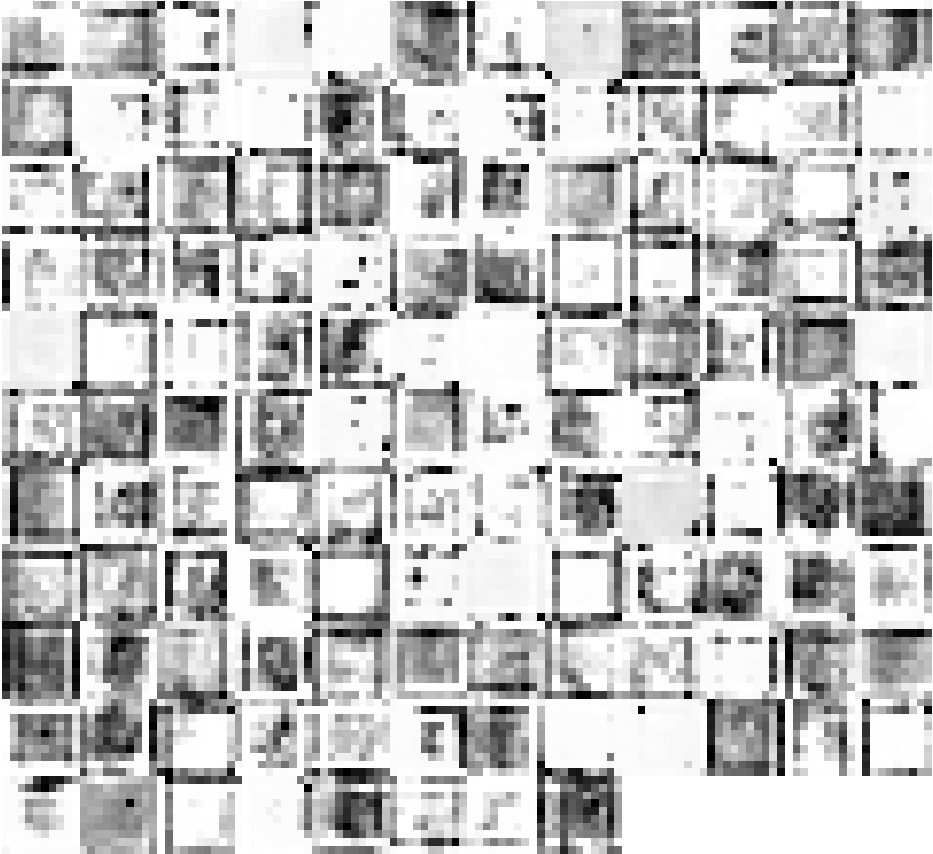
\includegraphics[width=\textwidth]{figures/galaxy_conv31.pdf}
    \caption{Layer 6 (128 maps$\times10\times10$)}
  \end{subfigure}
  \caption{
    (a) A sample $44\times44$ RGB image of a galaxy in the CFHTLenS data set.
    The RGB image is created by mapping R $\rightarrow i$ band magnitude,
    G $\rightarrow r$ band magnitude, and B $\rightarrow g$ band magnitude.
    (b) Activations on the first convolutional layer when a $5\times44\times44$
    image is fed into the network.
    (c) Activations on the third convolutional layer.
    (d) Activations on the sixth convolutional layer.
    Each image in (a), (b), and (c) is a feature map corresponding to the
    output for one of the learned features.
    }
  \label{fig:galaxy_activations}
\end{figure*}


\begin{figure*}
  \centering
  \begin{subfigure}[c]{0.24\linewidth}
  \centering
    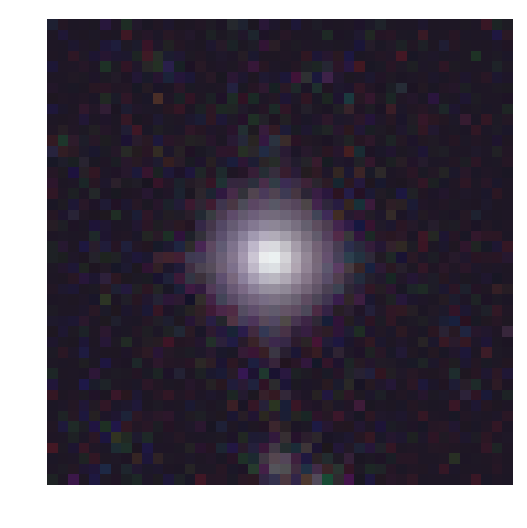
\includegraphics[width=\textwidth]{figures/star_original.pdf}
    \caption{Input (5 bands$\times44\times44$)}
  \end{subfigure}
  \hfill
  \begin{subfigure}[c]{0.24\linewidth}
  \centering
    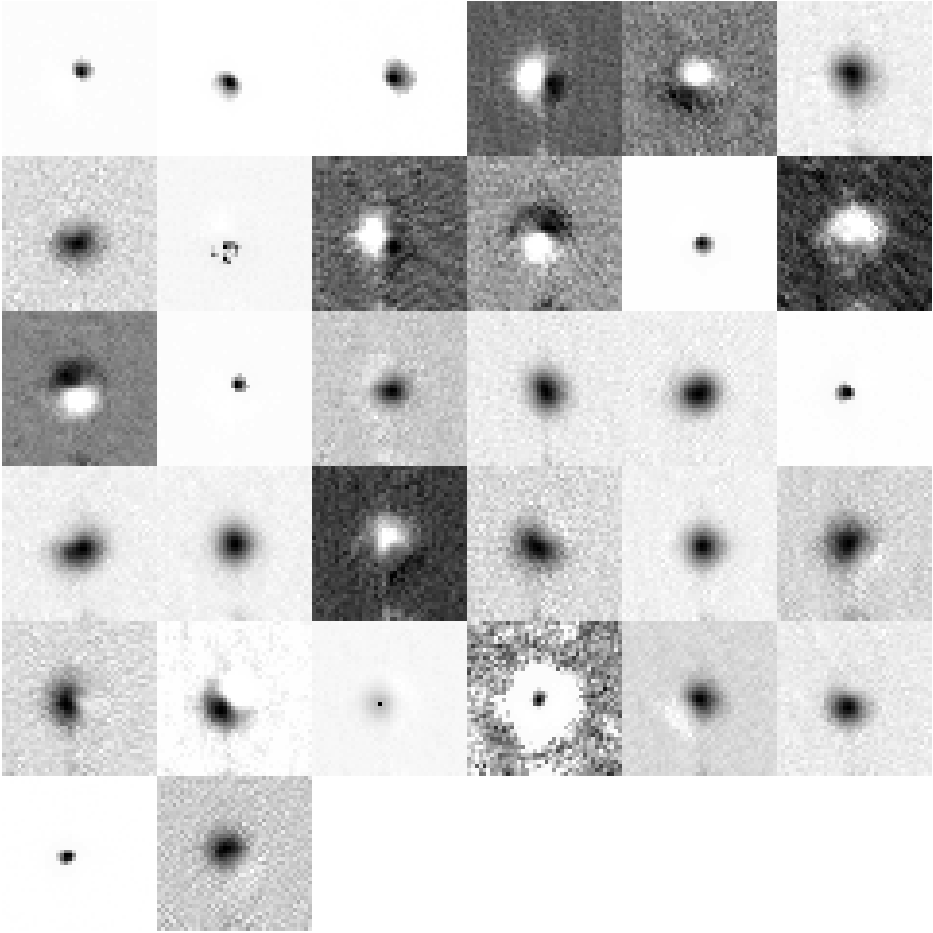
\includegraphics[width=\textwidth]{figures/star_conv11.pdf}
    \caption{Layer 1 (32 maps$\times40\times40$)}
  \end{subfigure}
  \hfill
  \begin{subfigure}[c]{0.24\linewidth}
  \centering
    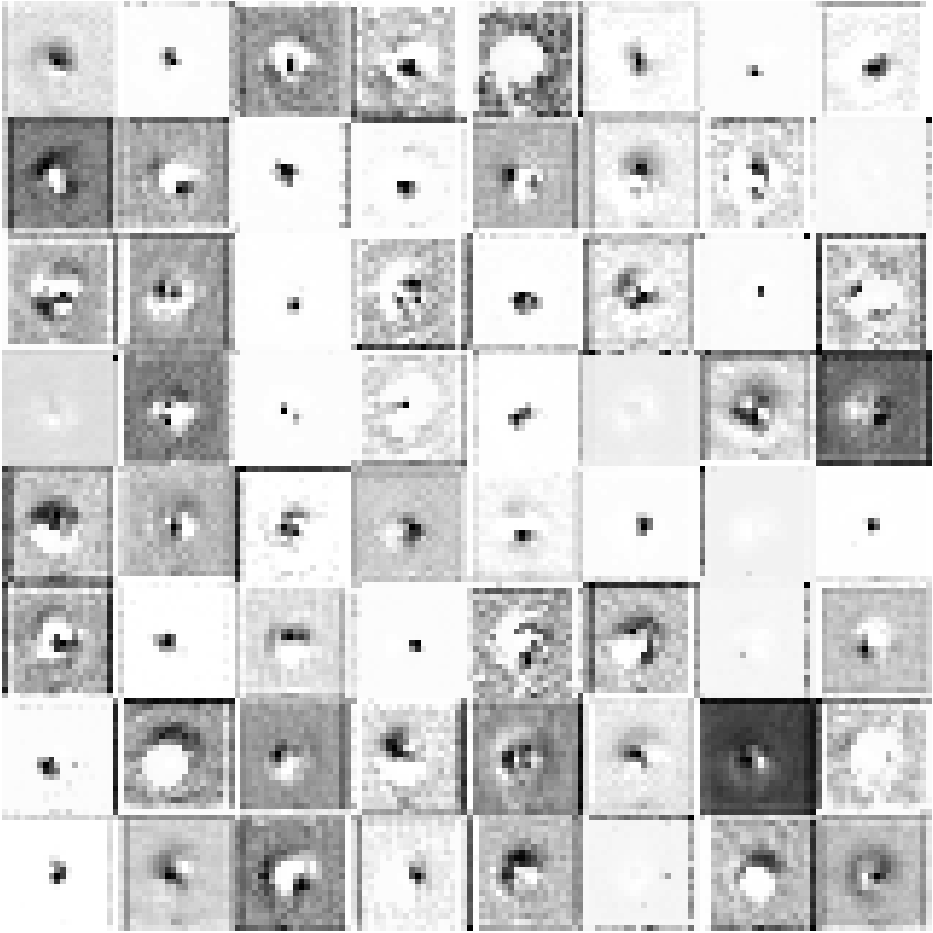
\includegraphics[width=\textwidth]{figures/star_conv21.pdf}
    \caption{Layer 3 (64 maps$\times20\times20$)}
  \end{subfigure}
  \hfill
  \begin{subfigure}[c]{0.24\linewidth}
  \centering
    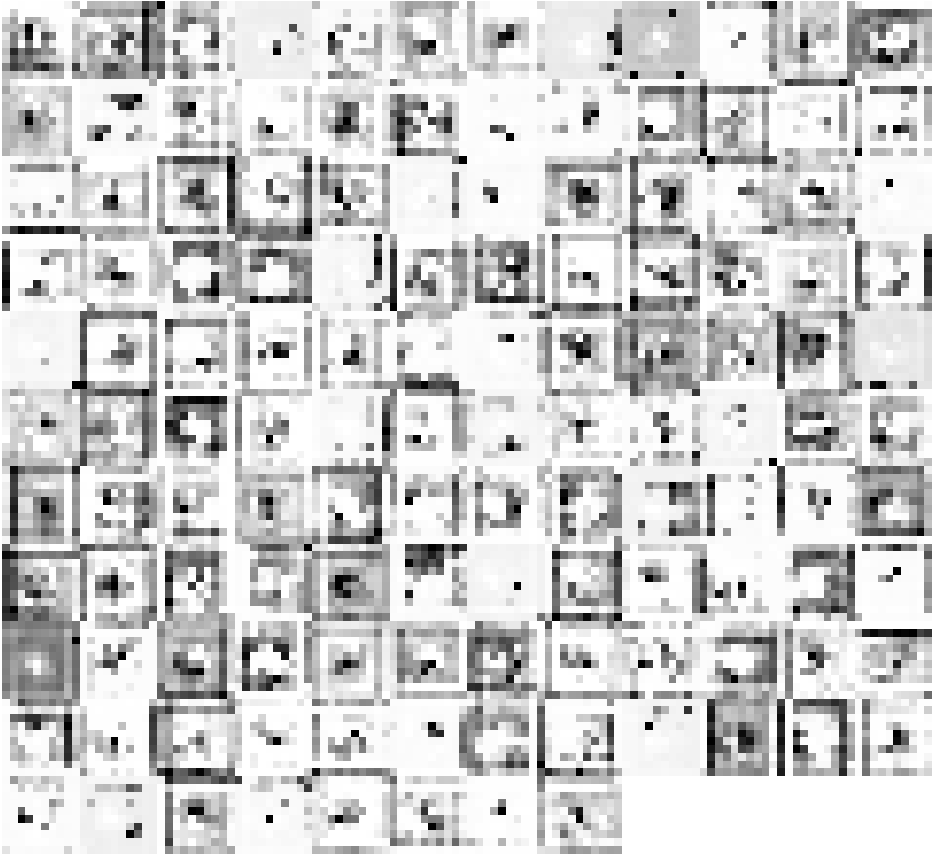
\includegraphics[width=\textwidth]{figures/star_conv31.pdf}
    \caption{Layer 6 (128 maps$\times10\times10$)}
  \end{subfigure}
  \caption{
    Similar to Figure~\ref{fig:galaxy_activations} but for a star in the
    CFHTLenS data set.
    }
  \label{fig:star_activations}
\end{figure*}

As described in Section~\ref{sec:convnet},
we train our ConvNet model by monitoring its performance on the validation set.

Figure~\ref{fig:clens_calibration_conv} shows the calibration curve
that compares $P_{\rmn{gal}}$,
the fraction of objects that are galaxies (as determined from their spectra),
to $P_{\rmn{conv}}$, the probabilistic output that our ConvNet model produces.


\subsection{SDSS}
  \label{sec:results_sdss}

\begin{table*}
  \caption{
    A summary of the classification performance metrics
    as applied to the SDSS data.
  }
  \centering
  \begin{tabular}{l c c c c c c}
    \hline
    classifier & AUC & MSE & $p_{g}(c_g=0.96) $ & $c_{s}(p_s=0.97)$ & CAL & $ |\Delta N_g|/N_g$ \\
    \hline
    ConvNet               & 0.9952          & 0.0182          & 0.9915          & 0.9500          & \textbf{0.0243} & 0.0157          \\
    TPC${}_{\rmn{morph}}$ & \textbf{0.9967} & \textbf{0.0099} & \textbf{0.9977} & \textbf{0.9810} & 0.0254          & \textbf{0.0044} \\
    TPC${}_{\rmn{phot}}$  & 0.9886          & 0.0283          & 0.9819          & 0.8879          & 0.0316          & 0.0160 \\
    \hline
  \end{tabular}
  \label{table:sdss_metrics}
\end{table*}


\begin{figure}
  \centering
  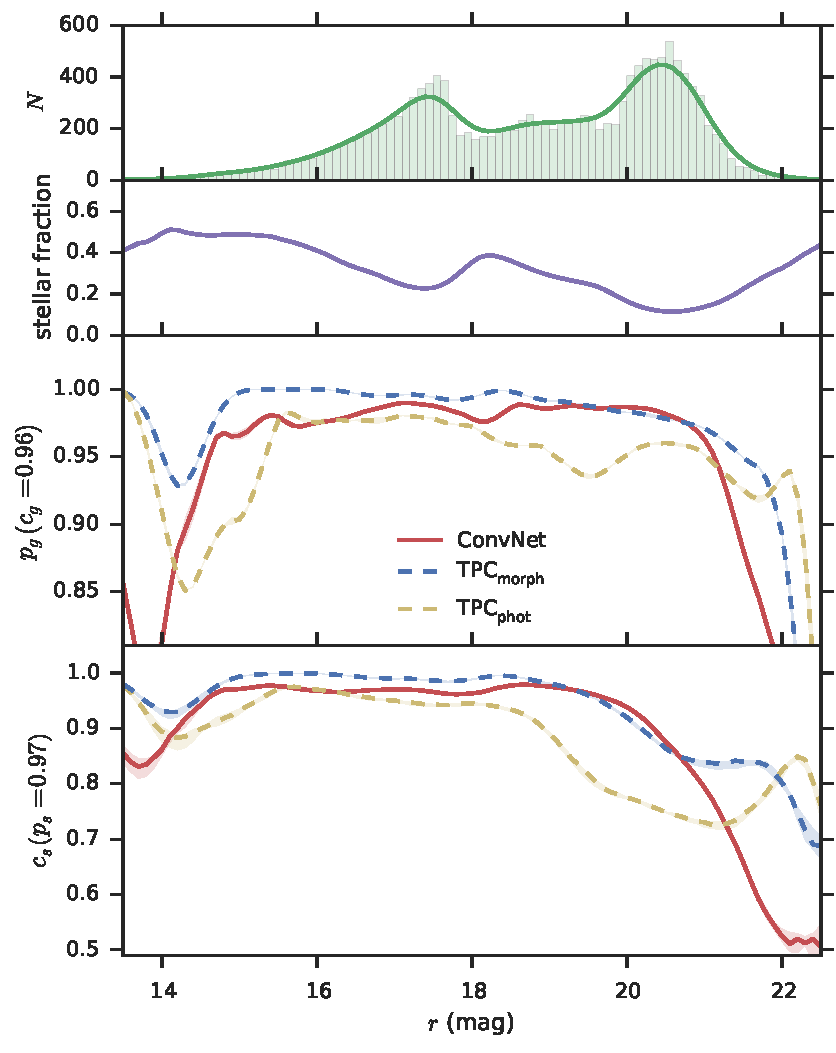
\includegraphics[width=\columnwidth]{figures/sdss_mag.pdf}
  \caption{Galaxy purity and star completeness as function of the $r$-band
    magnitude for the differential counts in the SDSS data set.}
  \label{fig:sdss_mag}
\end{figure}

\begin{figure}
  \centering
  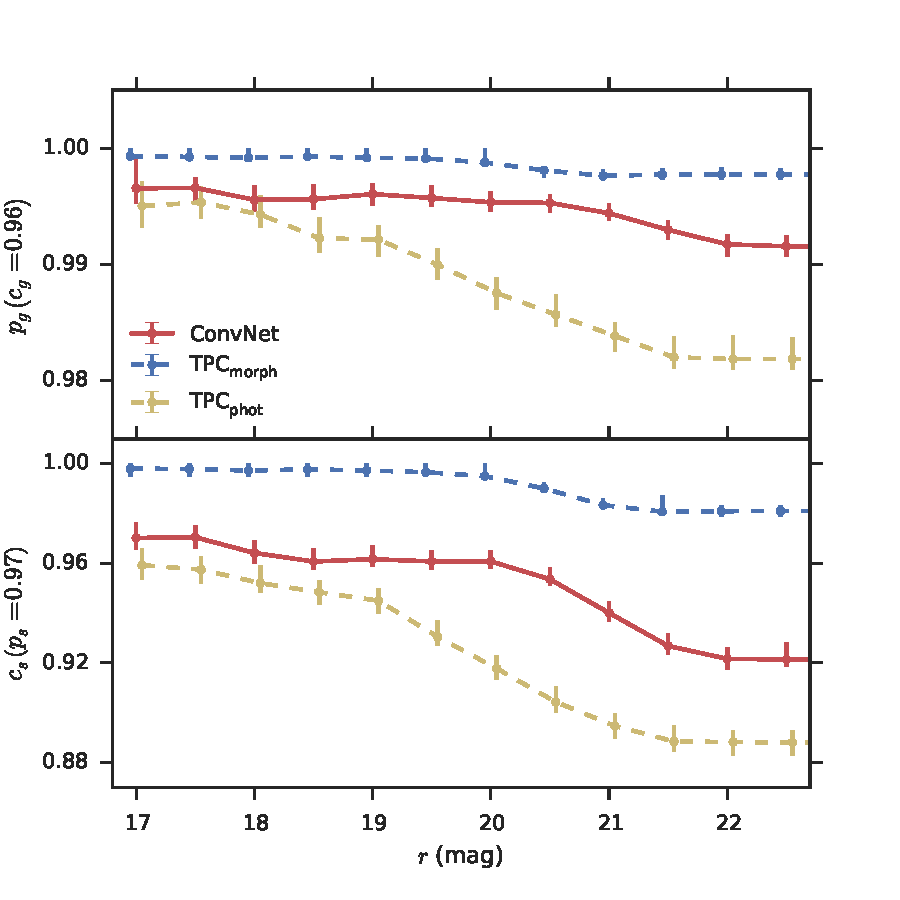
\includegraphics[width=\columnwidth]{figures/sdss_integrated.pdf}
  \caption{Galaxy purity and star completeness as functions of the $r$-band
    magnitude for the integrated counts in the SDSS data set.}
  \label{fig:sdss_integrated}
\end{figure}

\begin{figure}
  \centering
  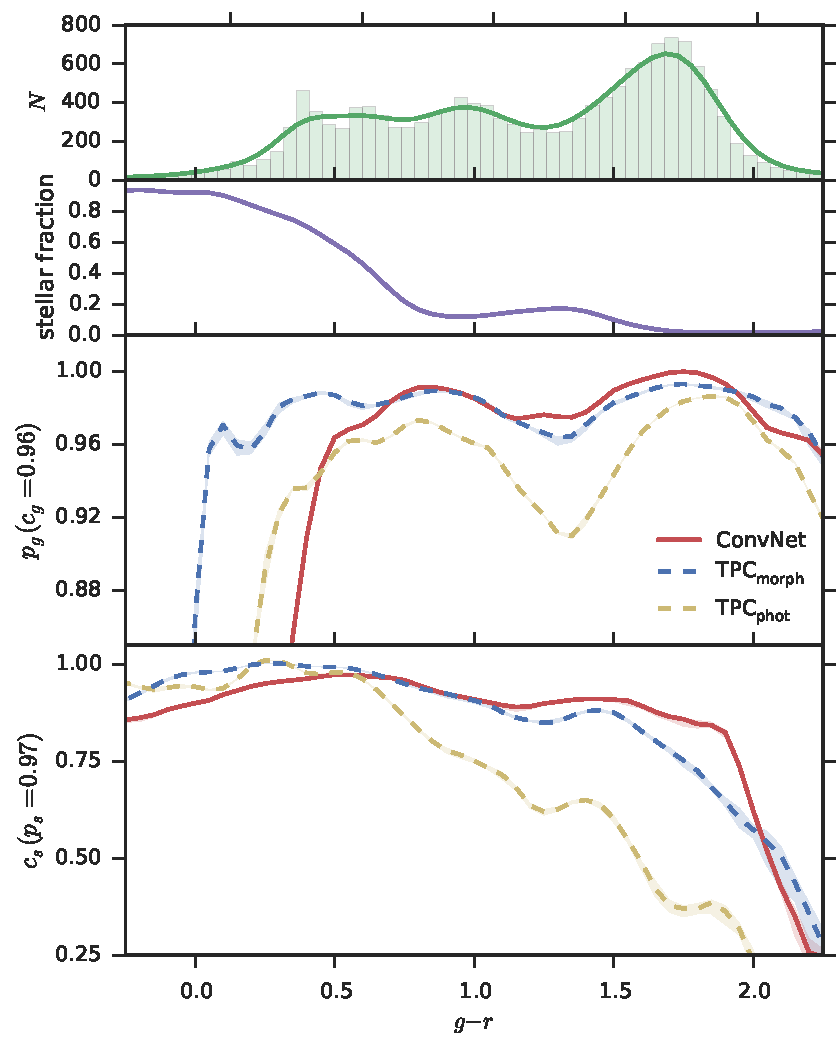
\includegraphics[width=\columnwidth]{figures/sdss_g_r.pdf}
  \caption{Similar to Figure~\ref{fig:sdss_mag} but as a function of
    $g-r$ color. The bin size of histogram in the top panel is 0.05.}
  \label{fig:sdss_g_r}
\end{figure}

\begin{figure*}
  \centering
  \begin{minipage}[c]{0.49\textwidth}
    \centering
    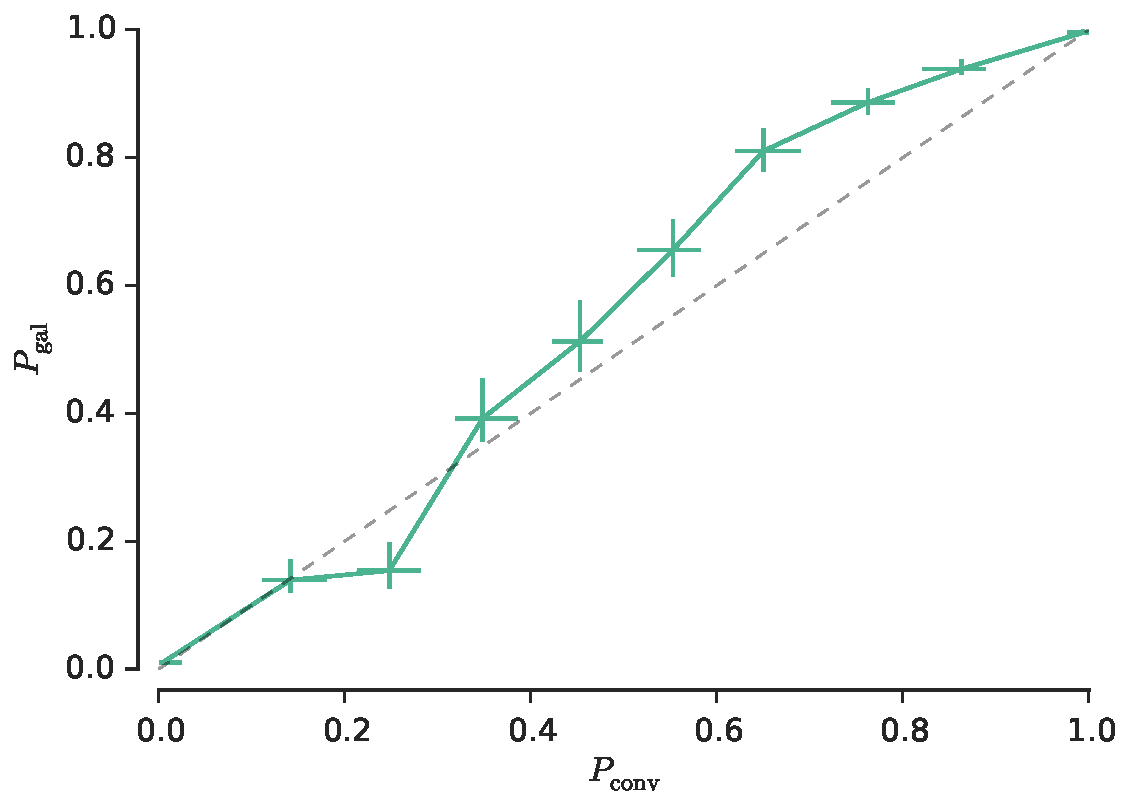
\includegraphics[width=\textwidth]{figures/sdss_calibration_conv.pdf}
    \caption{Calibration curve for ConvNet as applied to the SDSS data set.}
    \label{fig:sdss_calibration_conv}
  \end{minipage}
  \hfill
  \begin{minipage}[c]{0.49\textwidth}
    \centering
    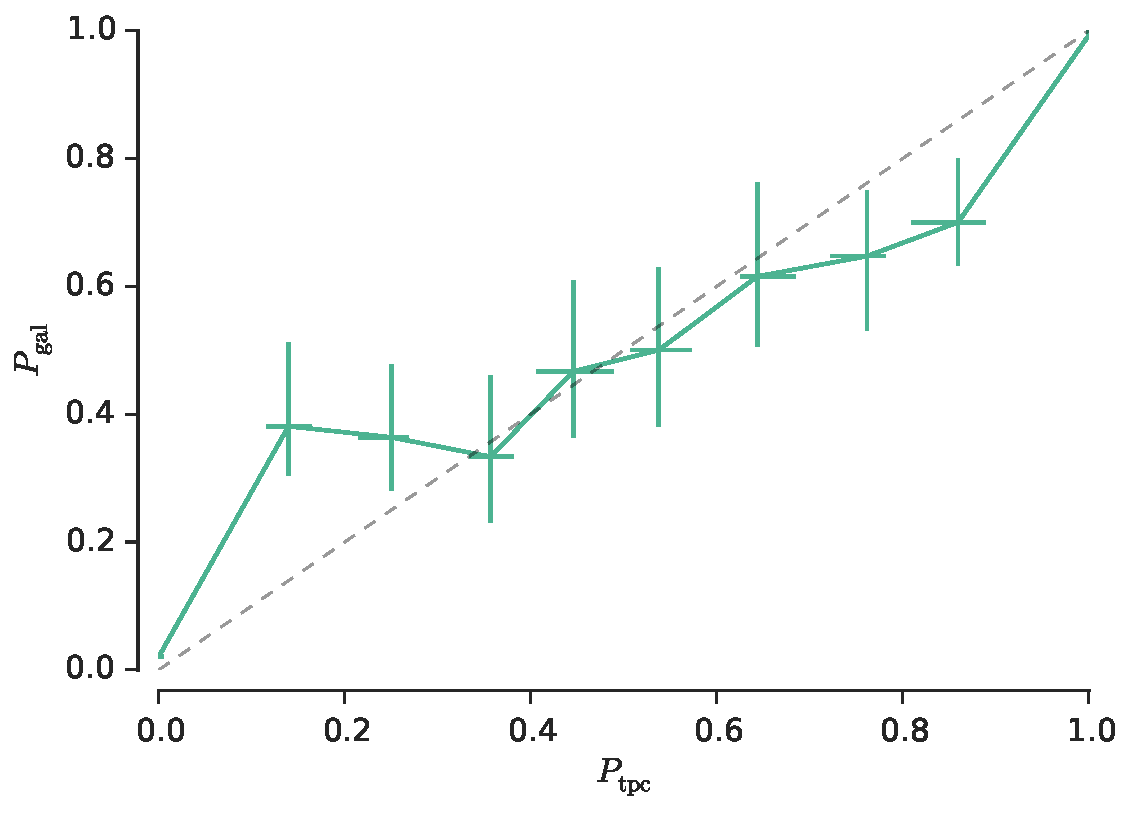
\includegraphics[width=\textwidth]{figures/sdss_calibration_tpc.pdf}
    \caption{Calibration curve for $\rmn{TPC}_{\rmn{morph}}$
      as applied to the SDSS data set.}
    \label{fig:sdss_calibration_tpc}
  \end{minipage}
\end{figure*}

We have also trained and tested our ConvNet model on the SDSS data set, and
we present in Table~\ref{table:sdss_metrics} the same six metrics for ConvNet,
$\rmn{TPC}_{\rmn{morph}}$, and $\rmn{TPC}_{\rmn{phot}}$.

In Figure~\ref{fig:sdss_mag}, we compare the galaxy purity
and star completeness values for ConvNet, $\rmn{TPC}_{\rmn{morph}}$, and
$\rmn{TPC}_{\rmn{phot}}$ as a
function of $r$-band magnitude for the differential counts in the SDSS data.


%%%%%%%%%%%%%%%%%%%%%%%%%%%%%%%%%%%%%%%%%%%%%%%%%%%%%%%%%%%%%%%%%%%%%%%%%%%%%%%%

\section{Conclusions}
  \label{sec:conclusions}

We have presented a convolutional neural network for classifying stars and
galaxies in the SDSS and CFHTLenS photometric images.


%%%%%%%%%%%%%%%%%%%%%%%%%%%%%%%%%%%%%%%%%%%%%%%%%%%%%%%%%%%%%%%%%%%%%%%%%%%%%%%%

\section*{Acknowledgements}

We acknowledge support from the 
National Science Foundation Grant No.\ AST-1313415.
RJB acknowledges support as an Associate
within the Center for Advanced Study at the University of Illinois.


This work used the Extreme Science and Engineering Discovery Environment
(XSEDE), which is supported by National Science Foundation grant number
ACI-1053575.

This work is based on observations obtained with MegaPrime/MegaCam, a
joint project of CFHT and CEA/DAPNIA, at the Canada-France-Hawaii
Telescope (CFHT) which is operated by the National Research Council
(NRC) of Canada, the Institut National des Sciences de l'Univers of
the Centre National de la Recherche Scientifique (CNRS) of France, and
the University of Hawaii. This research used the facilities of the
Canadian Astronomy Data Centre operated by the National Research
Council of Canada with the support of the Canadian Space Agency.
CFHTLenS data processing was made possible thanks to significant
computing support from the NSERC Research Tools and Instruments grant
program.

Funding for SDSS-III has been provided by the Alfred P. Sloan Foundation, the
Participating Institutions, the National Science Foundation, and the U.S.
Department of Energy Office of Science. The SDSS-III web site is
http://www.sdss3.org/.

SDSS-III is managed by the Astrophysical Research Consortium for the
Participating Institutions of the SDSS-III Collaboration including the
University of Arizona, the Brazilian Participation Group, Brookhaven National
Laboratory, Carnegie Mellon University, University of Florida, the French
Participation Group, the German Participation Group, Harvard University, the
Instituto de Astrofisica de Canarias, the Michigan State/Notre Dame/JINA
Participation Group, Johns Hopkins University, Lawrence Berkeley National
Laboratory, Max Planck Institute for Astrophysics, Max Planck Institute for
Extraterrestrial Physics, New Mexico State University, New York University,
Ohio State University, Pennsylvania State University, University of Portsmouth,
Princeton University, the Spanish Participation Group, University of Tokyo,
University of Utah, Vanderbilt University, University of Virginia, University
of Washington, and Yale University.

\footnotesize{
\bibliographystyle{mnras}
\bibliography{sg_paper}
}

% Don't change these lines
\bsp	% typesetting comment
\label{lastpage}
\end{document}

% End of mnras_template.tex
